\begin{enumerate}
\item Sign Up\par

To Sign up, insert your details in the following box on our Home page.
To sign up for an account, and get a User ID, enter user details in the appropriate fields on our Home page in the following figure.\par

 \begin{figure}[H] 
	\centering
	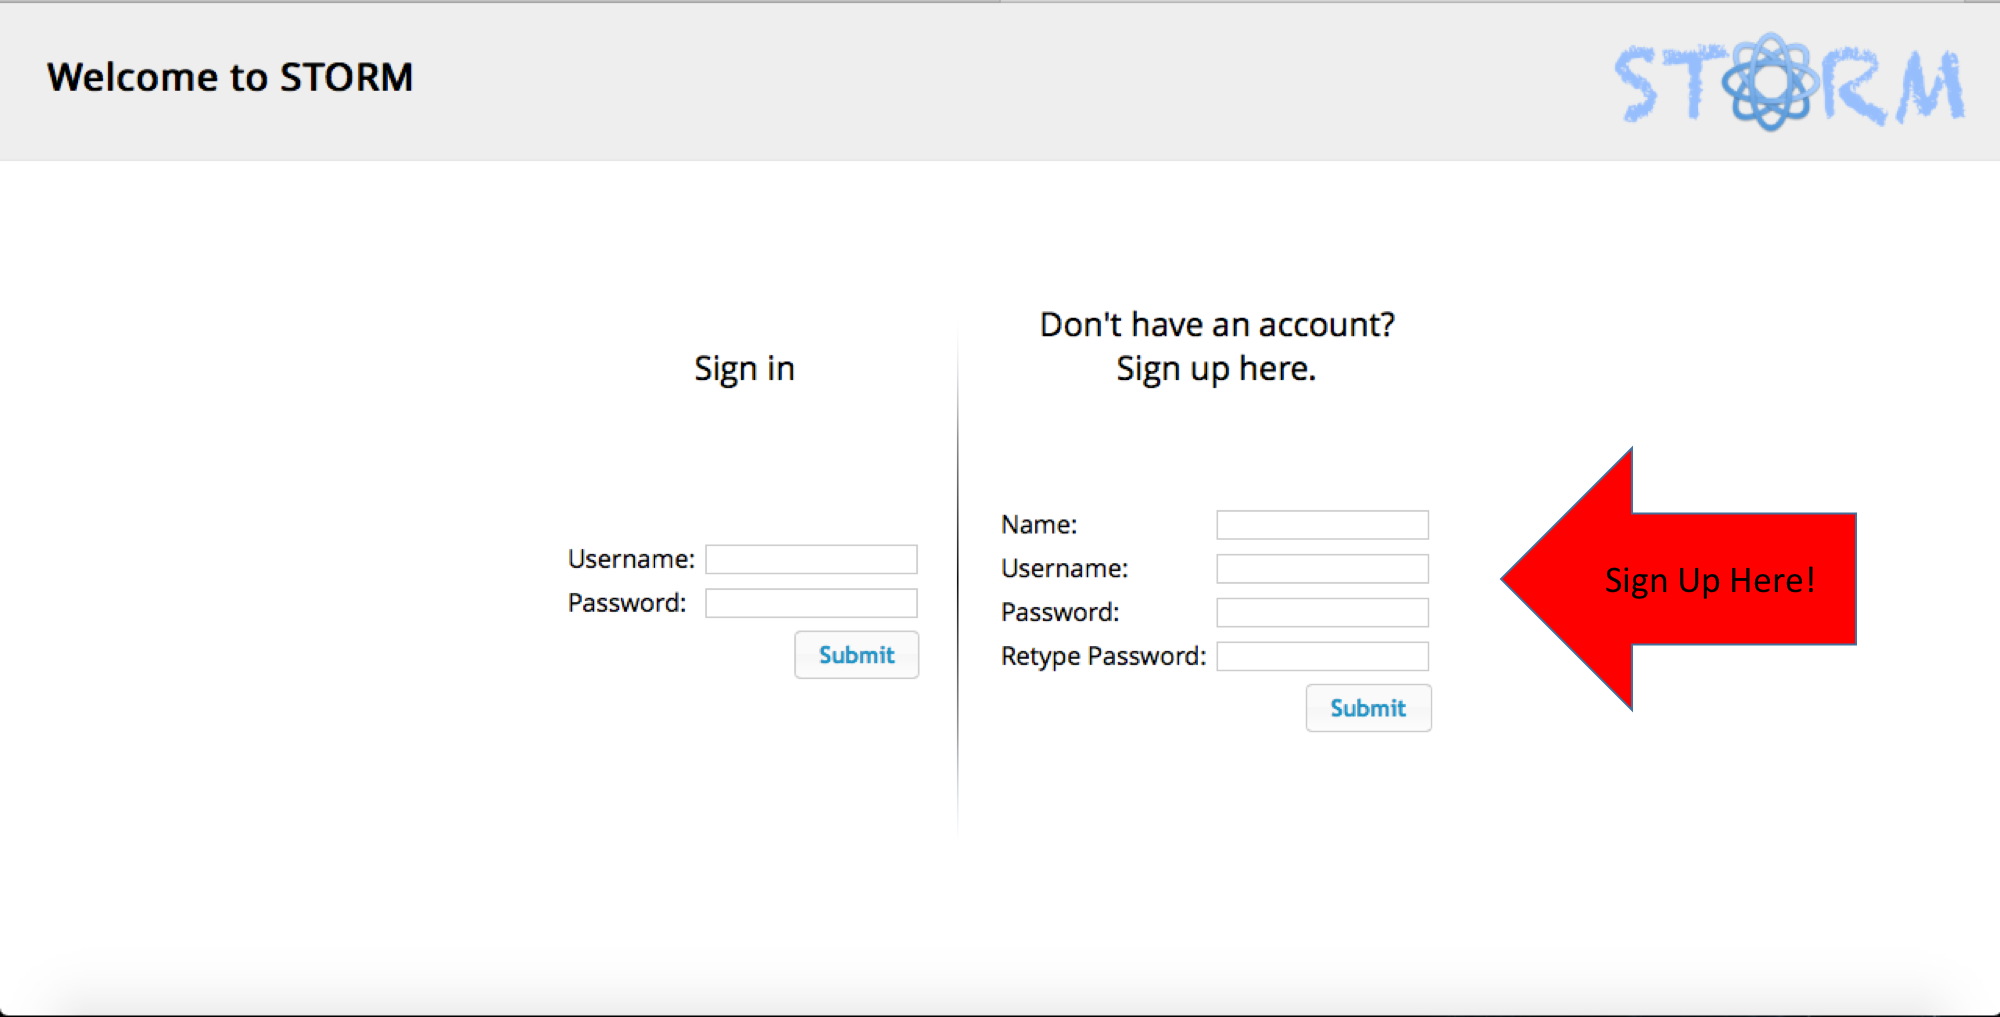
\includegraphics[width=6cm]{./graphics/StormUMSU1.jpg}\par
	\caption{Signing Up to STORM}
\end{figure}
Click on submit and the system will register the user in the database.

\item Login\par
To log in to an account enter user details in the appropriate fields in the following figure.\par
 \begin{figure}[H] 
	\centering
	
\includegraphics[width=13cm]{./graphics/StormUMSU2.jpg}\par
	\caption{Logging in to STORM}
\end{figure}
Click on submit and the system will navigate to the user's specific team shuffling page.

\item Log out\par
Logging out of your account can be achieved by simply clicking on the "Logout" button that will be displayed at the upper right corner of your screen after being logged in.
 \begin{figure}[H] 
	\centering
	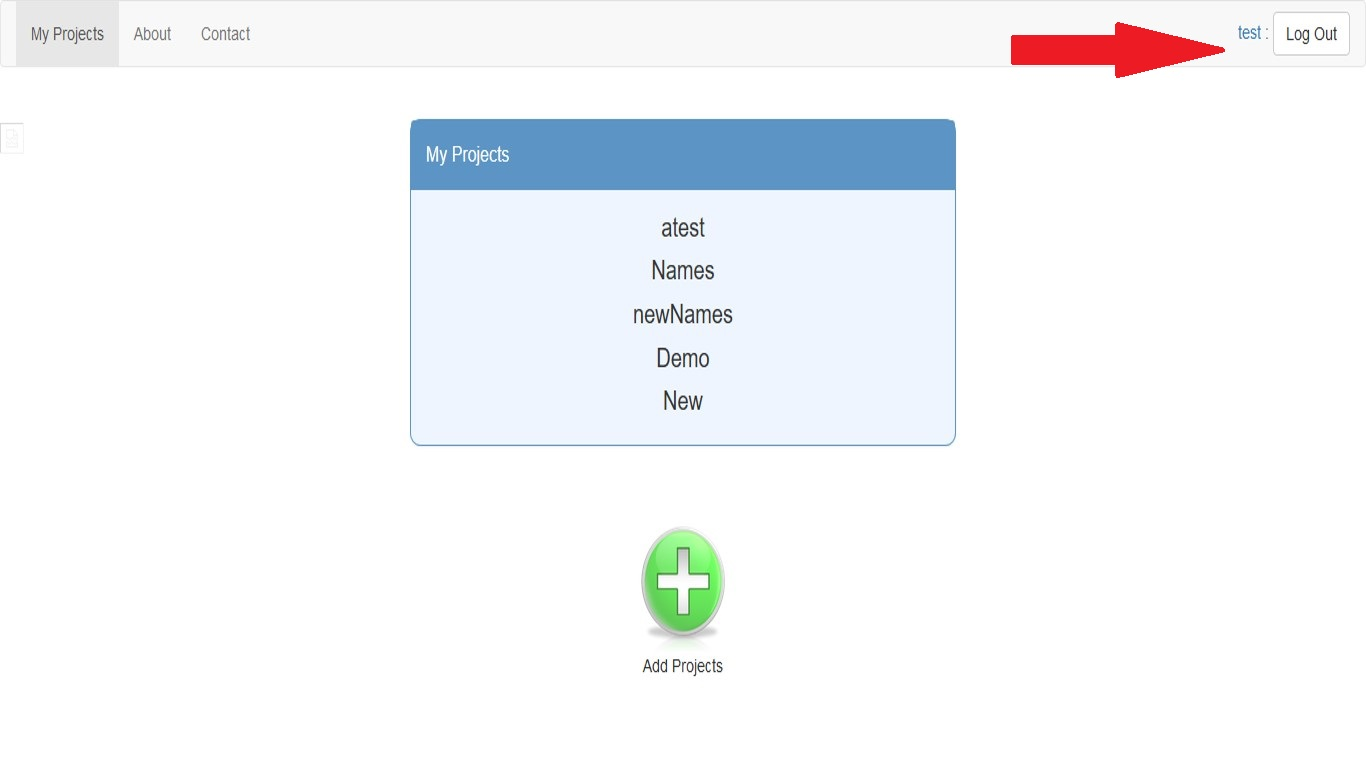
\includegraphics[width=13cm]{./graphics/Logout.jpg}\par
	\caption{Logging out of STORM}
\end{figure}

\item Team Setup\par
The first page you will see after logging in, will be the Team Setup page.  Where you can manage all the teams that you have created with the software.\par
 \begin{figure}[H] 
	\centering
	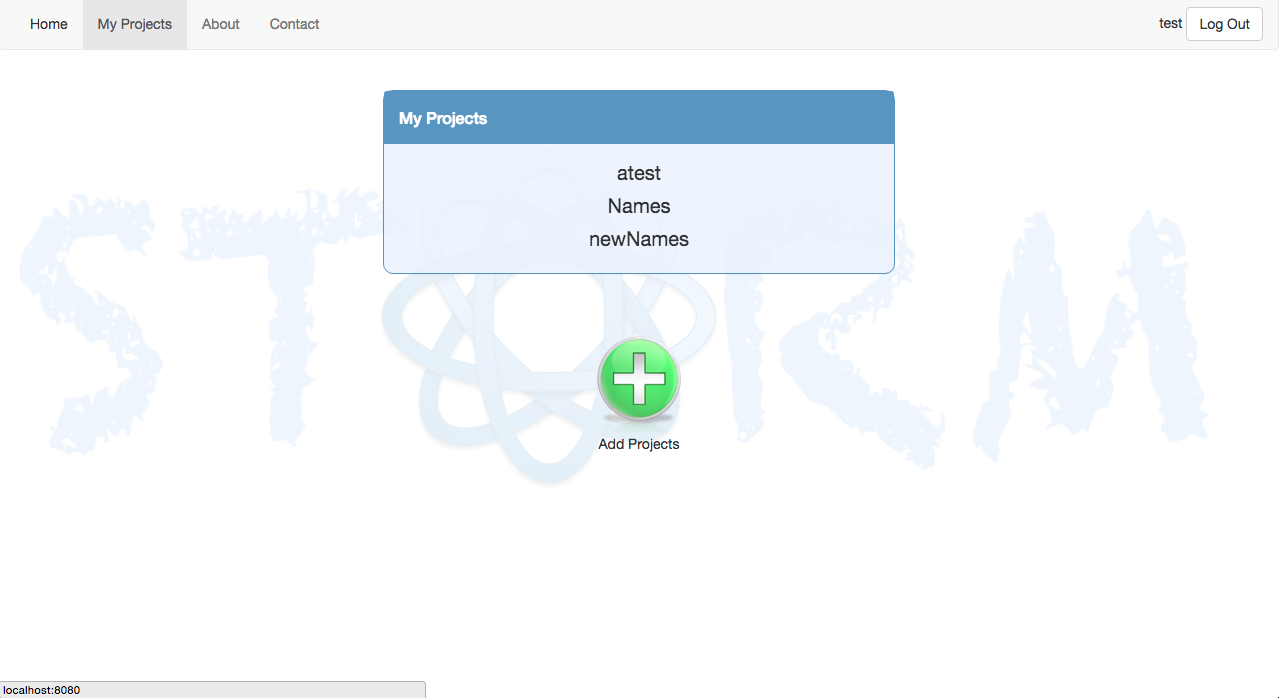
\includegraphics[width=13cm]{./graphics/TeamSetup.jpg}\par
	\caption{Team Setup Page}
\end{figure}

\item Shuffle\par
After choosing a team to work with, the following page will be displayed.  Here you can see the team you have created, or start by creating your first team dynamically by using the options at the top of the page.\par
 \begin{figure}[H] 
	\centering
	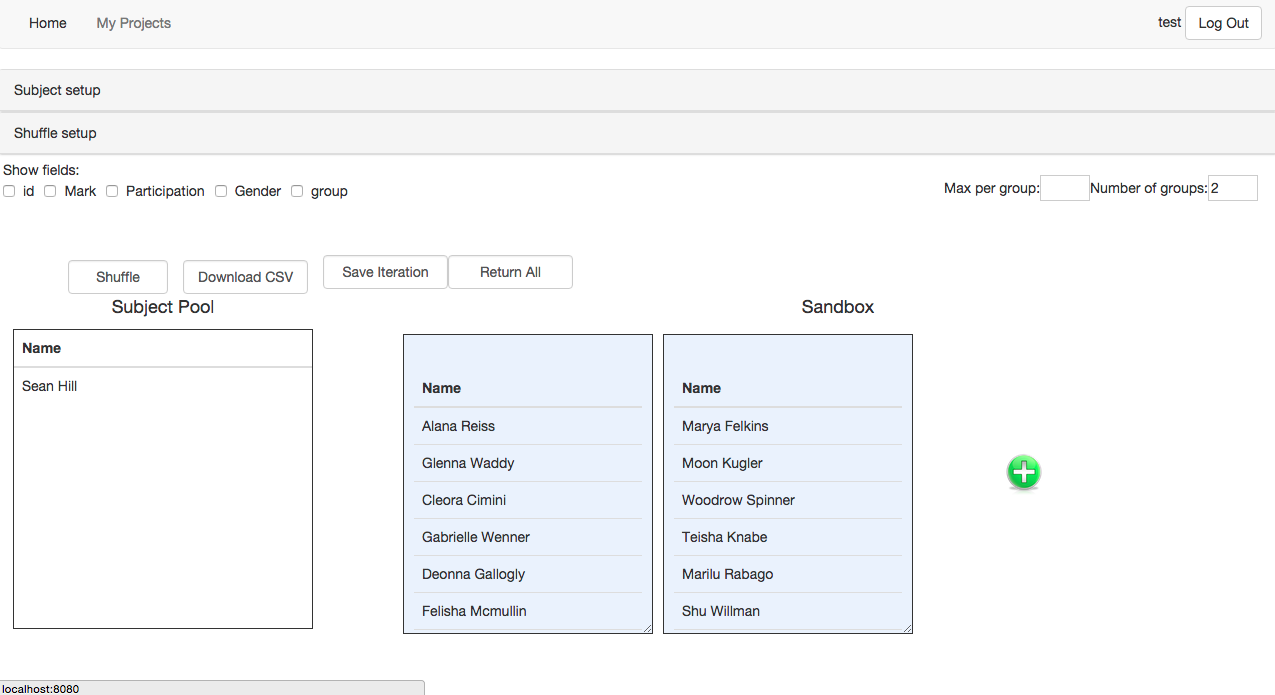
\includegraphics[width=13cm]{./graphics/Shuffle.jpg}\par
	\caption{Shuffling Page}
\end{figure}

\newpage
\item Subject Setup\par
This options tab allows users to review their subject data. All the data uploaded to the database are showed here. You can add subjects, delete subjects or edit subjects.\par
 \begin{figure}[H] 
	\centering
	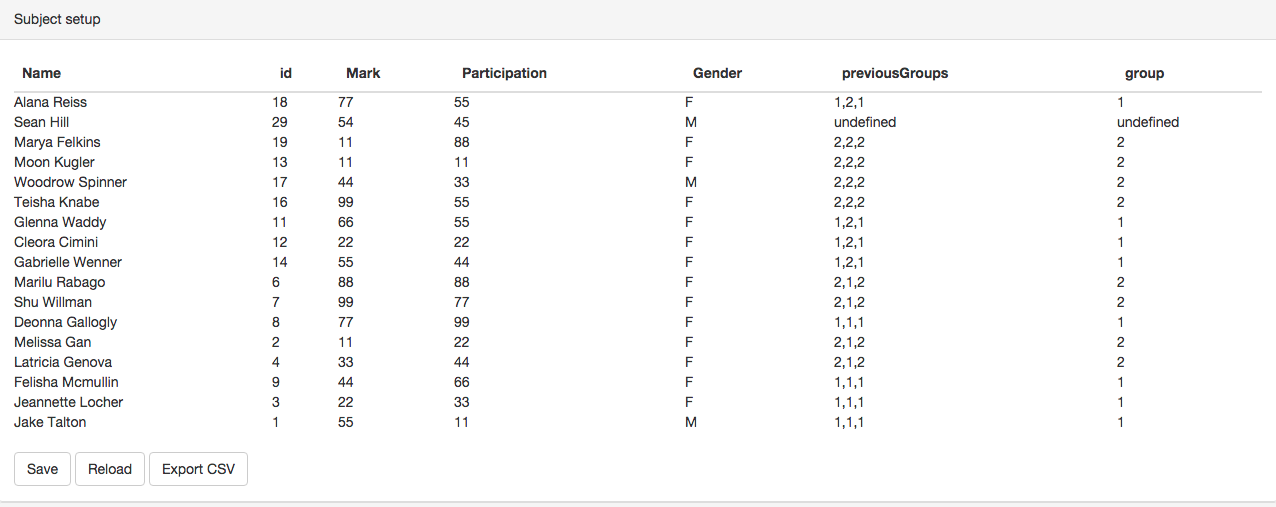
\includegraphics[width=13cm]{./graphics/SubjectSetup.jpg}\par
	\caption{Subject Setup dropdown}
\end{figure}
\begin{figure}[H] 
	\centering
	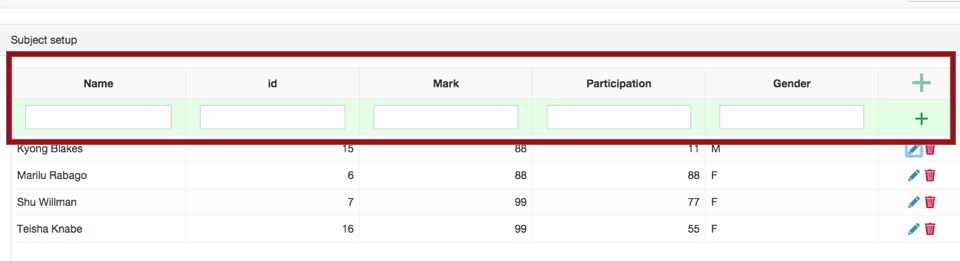
\includegraphics[width=13cm]{./graphics/AddManualSubject.jpg}\par
	\caption{Add Manual Subject}
\end{figure}
 \begin{figure}[H] 
	\centering
	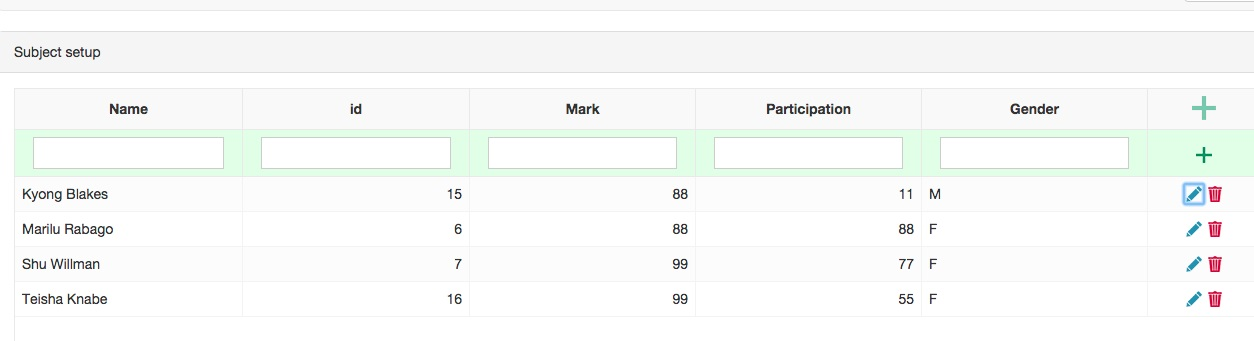
\includegraphics[width=13cm]{./graphics/EditAndDeleteSubject.jpg}\par
	\caption{Edit and Delete Subjects}
\end{figure}

\item Shuffle Setup\par
This options tab allows users to make choices about the shuffling algorithm to use, as well as the weights of criteria in multi criteria shuffles.\par
 \begin{figure}[H] 
	\centering
	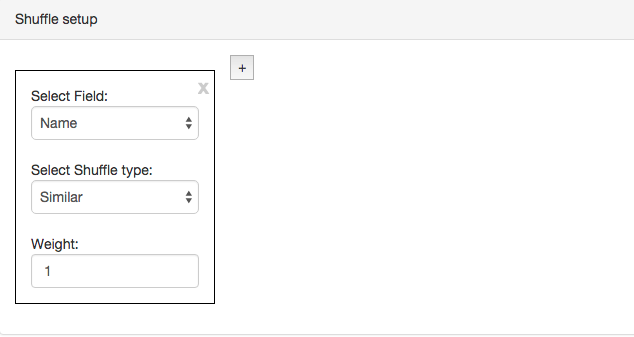
\includegraphics[width=13cm]{./graphics/ShuffleSetup.jpg}\par
	\caption{Shuffle Setup dropdown}
\end{figure}

\item Upload CSV\par
A .csv file can be uploaded into the system after a project has been created to add more subjects and criteria to the project. Firstly export the .csv from STORM, update the .csv and import the .csv as can be seen using the buttons in the figure below.\par
 \begin{figure}[H] 
	\centering
	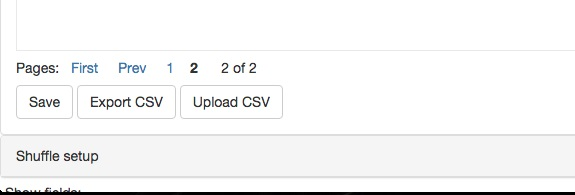
\includegraphics[width=13cm]{./graphics/UploadCSV.jpg}\par
	\caption{Shuffle Setup dropdown}
\end{figure}
\begin{itemize}
	\item The following rules apply to uploading the initial .csv
	\begin{enumerate}
		\item The file cannot be empty
		\item The file must contain at least 2 columns 
		\item The file must contain at least 2 subjects
		\item The first Row must be column headers(Criteria names)
		\item One of the columns must be a unique identifier and have a unique value for every subject.
		\item The unique identifier column must be the first column.
		\item Each student must contain a value for each column.
		\item Any number of columns can be present
		\item Any number of subjects can be present
		\item Values may not contain instances of “;” or “,” characters.
		\item The second column must contain subject names with header ‘Names’ as this value is the default value to 				display subjects in the team setup shuffling page.
	\end{enumerate}
 \begin{figure}[H] 
	\centering
	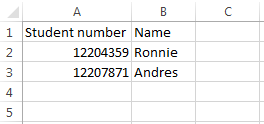
\includegraphics[width=13cm]{./graphics/MinInitial.png}\par
	\caption{Minimal Initial Upload}
\end{figure}
 \begin{figure}[H] 
	\centering
	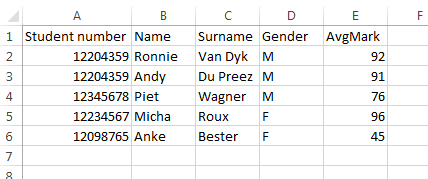
\includegraphics[width=13cm]{./graphics/CorrectInitial.png}\par
	\caption{Correct Initial Upload}
\end{figure}
 \begin{figure}[H] 
	\centering
	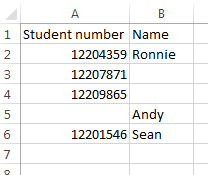
\includegraphics[width=7cm]{./graphics/IncorrectInitial.png}\par
	\caption{Incorrect Initial Upload Example - Rules (b) \& (c) Broken}
\end{figure}
 \begin{figure}[H] 
	\centering
	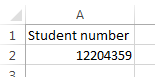
\includegraphics[width=7cm]{./graphics/IncorrectInitial1.png}\par
	\caption{Incorrect Initial Upload Example - Rule (g) Broken}
\end{figure}
	\item The following rules apply to uploading additional .csv files
	\begin{enumerate}
		\item[] \textit{All initial upload rules apply to any additional uploads, except for rule (c).}
		\item Hints
		\begin{enumerate}
			\item Download a csv containing all subjects in the current set.
			\item Add additional criteria or subjects to that file. 
			\item Subjects can also be edited and the changed values will overwrite the current values in the set.
			\item Do not delete a subject from the file(Deleting subjects can be done online in the subjects table)
		\end{enumerate}
		\item Rules for adding criteria
		\begin{enumerate}
			\item First column of the file must contain unique identifiers, one for each subject currently existing in the 					set. (Omitting one identifier will result in error)
			\item New criteria can be added in the column next to the identifiers. (Omitting the rest of the columns 					currently in the set. This is to make it possible for the user to add criteria by using only a list of all the 					subject’s unique identifiers. NB no additional subjects can be added in this way. See ‘Adding Criteria and 					Subjects’ section. More than one new criteria can also be added in this way.)
		\end{enumerate}
	
	\begin{figure}[H] 
	\centering
	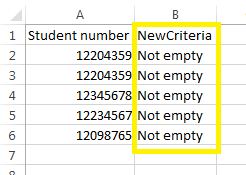
\includegraphics[width=8cm]{./graphics/AddCr.png}\par
	\caption{Correct add criteria upload}
	\end{figure}
	\item Rules for adding subjects
	\begin{enumerate}
		\item For only adding new subjects use the whole subject set. (can be downloaded from the team setup page) and 			append new students at the end of the file.
		\item New subjects must have a value for each criteria currently in the set.
		\item New subjects must have an identifier unique from any existing subjects in the set.
	\end{enumerate}
	\begin{figure}[H] 
	\centering
	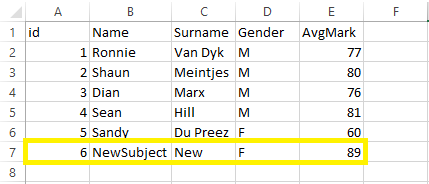
\includegraphics[width=13cm]{./graphics/AddSub.png}\par
	\caption{Correct add subjects upload}
	\end{figure}
	\item Rules for adding subjects and criteria (Growing the set horizontally and vertically)
	\begin{enumerate}
		\item For only adding new criteria and subjects use the whole subject set. (can be downloaded from the team setup 		page)
		\item Append new criteria in the first available column next to the last criteria in the current set.
		\item Append subjects to the end of the file after the last subject in the current set.
		\item New students must have values for each criteria in the current set, even newly added criteria.
	\end{enumerate}
\end{enumerate}
	\begin{figure}[H] 
	\centering
	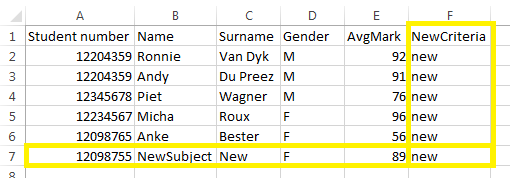
\includegraphics[width=13cm]{./graphics/AddSubCrit.png}\par
	\caption{Correct add subjects and criteria upload}
	\end{figure}

\end{itemize}
\end{enumerate}


